\chapter{Результаты и выводы}	% Заголовок

\section*{Результаты}

В ходе работы был создан расширяемый программный пакет. Он масштабируем в смысле расширения его функциональных возможностей (поддерживаемых классов распределений, моделей копул, форматов обмена данными). С его помощью было построено 243 аппроксимации копулы (для каждой пары параметров и их значений). Каждая такая оценка была визуализирована для анализа качественных и количественных характеристик результатов интервального оценивания, полученных композицией алгоритмов из работы [Сидоровская, 2015].

В качестве асимптотической оценки таких двумерных распределений, при условии, что алгоритмы интервального оценивания обеспечивают состоятельные оценки границ компактов, ожидается получить плотности копулы $\Pi$. Это было бы свидетельством того факта, что попадание или не попадание модельного значения одного параметра в его компакт никак не связано с аналогичными исходами интервального оценивания по другим параметрам. Но исследование показало, что это не так.

Между исходами интервального оценивания границ компактов присутствуют стохастические связи.
%% опять речь о $\xi$, который нигде выше формально не определили
Это справедливо только для интервальных оценок, доставляемых алгоритмом с вектором параметров $\overline{\xi}$. На основе оценок плотностей копул, полученных в этой работе, следует отобрать пары параметров и значений, на которые следует обращать внимание при последующей работе с алгоритмом оценивания. Возможно, удастся добиться построения таких оценок, для которых вероятности попадания будут независимы.


\section*{Выводы}

В качестве примера выберем для анализа пару параметров $\sigma$ и $x_m$.
\begin{figure}[h]
	{% GNUPLOT: LaTeX picture with Postscript
\begingroup
  \makeatletter
  \providecommand\color[2][]{%
    \GenericError{(gnuplot) \space\space\space\@spaces}{%
      Package color not loaded in conjunction with
      terminal option `colourtext'%
    }{See the gnuplot documentation for explanation.%
    }{Either use 'blacktext' in gnuplot or load the package
      color.sty in LaTeX.}%
    \renewcommand\color[2][]{}%
  }%
  \providecommand\includegraphics[2][]{%
    \GenericError{(gnuplot) \space\space\space\@spaces}{%
      Package graphicx or graphics not loaded%
    }{See the gnuplot documentation for explanation.%
    }{The gnuplot epslatex terminal needs graphicx.sty or graphics.sty.}%
    \renewcommand\includegraphics[2][]{}%
  }%
  \providecommand\rotatebox[2]{#2}%
  \@ifundefined{ifGPcolor}{%
    \newif\ifGPcolor
    \GPcolortrue
  }{}%
  \@ifundefined{ifGPblacktext}{%
    \newif\ifGPblacktext
    \GPblacktextfalse
  }{}%
  % define a \g@addto@macro without @ in the name:
  \let\gplgaddtomacro\g@addto@macro
  % define empty templates for all commands taking text:
  \gdef\gplbacktext{}%
  \gdef\gplfronttext{}%
  \makeatother
  \ifGPblacktext
    % no textcolor at all
    \def\colorrgb#1{}%
    \def\colorgray#1{}%
  \else
    % gray or color?
    \ifGPcolor
      \def\colorrgb#1{\color[rgb]{#1}}%
      \def\colorgray#1{\color[gray]{#1}}%
      \expandafter\def\csname LTw\endcsname{\color{white}}%
      \expandafter\def\csname LTb\endcsname{\color{black}}%
      \expandafter\def\csname LTa\endcsname{\color{black}}%
      \expandafter\def\csname LT0\endcsname{\color[rgb]{1,0,0}}%
      \expandafter\def\csname LT1\endcsname{\color[rgb]{0,1,0}}%
      \expandafter\def\csname LT2\endcsname{\color[rgb]{0,0,1}}%
      \expandafter\def\csname LT3\endcsname{\color[rgb]{1,0,1}}%
      \expandafter\def\csname LT4\endcsname{\color[rgb]{0,1,1}}%
      \expandafter\def\csname LT5\endcsname{\color[rgb]{1,1,0}}%
      \expandafter\def\csname LT6\endcsname{\color[rgb]{0,0,0}}%
      \expandafter\def\csname LT7\endcsname{\color[rgb]{1,0.3,0}}%
      \expandafter\def\csname LT8\endcsname{\color[rgb]{0.5,0.5,0.5}}%
    \else
      % gray
      \def\colorrgb#1{\color{black}}%
      \def\colorgray#1{\color[gray]{#1}}%
      \expandafter\def\csname LTw\endcsname{\color{white}}%
      \expandafter\def\csname LTb\endcsname{\color{black}}%
      \expandafter\def\csname LTa\endcsname{\color{black}}%
      \expandafter\def\csname LT0\endcsname{\color{black}}%
      \expandafter\def\csname LT1\endcsname{\color{black}}%
      \expandafter\def\csname LT2\endcsname{\color{black}}%
      \expandafter\def\csname LT3\endcsname{\color{black}}%
      \expandafter\def\csname LT4\endcsname{\color{black}}%
      \expandafter\def\csname LT5\endcsname{\color{black}}%
      \expandafter\def\csname LT6\endcsname{\color{black}}%
      \expandafter\def\csname LT7\endcsname{\color{black}}%
      \expandafter\def\csname LT8\endcsname{\color{black}}%
    \fi
  \fi
    \setlength{\unitlength}{0.0500bp}%
    \ifx\gptboxheight\undefined%
      \newlength{\gptboxheight}%
      \newlength{\gptboxwidth}%
      \newsavebox{\gptboxtext}%
    \fi%
    \setlength{\fboxrule}{0.5pt}%
    \setlength{\fboxsep}{1pt}%
\begin{picture}(9070.00,4534.00)%
    \gplgaddtomacro\gplbacktext{%
    }%
    \gplgaddtomacro\gplfronttext{%
      \csname LTb\endcsname%
      \put(2863,4030){\makebox(0,0)[r]{\strut{}$\widehat{p}_\sigma=2.12132$, $\widehat{p}_\lambda=15$}}%
      \csname LTb\endcsname%
      \put(683,1188){\makebox(0,0){\strut{}\ft $0$}}%
      \put(1067,1084){\makebox(0,0){\strut{}\ft $0.2$}}%
      \put(1451,979){\makebox(0,0){\strut{}\ft $0.4$}}%
      \put(1835,875){\makebox(0,0){\strut{}\ft $0.6$}}%
      \put(2219,771){\makebox(0,0){\strut{}\ft $0.8$}}%
      \put(2602,667){\makebox(0,0){\strut{}\ft $1$}}%
      \put(1436,797){\makebox(0,0){\strut{}$\widehat{p}_\sigma$}}%
      \put(2787,710){\makebox(0,0){\strut{}\ft $0$}}%
      \put(3008,891){\makebox(0,0){\strut{}\ft $0.2$}}%
      \put(3230,1071){\makebox(0,0){\strut{}\ft $0.4$}}%
      \put(3452,1252){\makebox(0,0){\strut{}\ft $0.6$}}%
      \put(3673,1433){\makebox(0,0){\strut{}\ft $0.8$}}%
      \put(3895,1613){\makebox(0,0){\strut{}\ft $1$}}%
      \put(3706,1083){\makebox(0,0){\strut{}$\widehat{p}_\lambda$}}%
      \put(627,1886){\makebox(0,0)[r]{\strut{}\ft $0$}}%
      \put(627,2168){\makebox(0,0)[r]{\strut{}\ft $3$}}%
      \put(627,2450){\makebox(0,0)[r]{\strut{}\ft $6$}}%
      \put(627,2733){\makebox(0,0)[r]{\strut{}\ft $9$}}%
      \put(627,3016){\makebox(0,0)[r]{\strut{}\ft $12$}}%
      \put(-171,2487){\makebox(0,0){\strut{}$\widehat{c}$}}%
    }%
    \gplgaddtomacro\gplbacktext{%
    }%
    \gplgaddtomacro\gplfronttext{%
      \csname LTb\endcsname%
      \put(5223,578){\makebox(0,0){\strut{}\ft $0$}}%
      \put(5855,578){\makebox(0,0){\strut{}\ft $0.2$}}%
      \put(6487,578){\makebox(0,0){\strut{}\ft $0.4$}}%
      \put(7117,578){\makebox(0,0){\strut{}\ft $0.6$}}%
      \put(7749,578){\makebox(0,0){\strut{}\ft $0.8$}}%
      \put(8381,578){\makebox(0,0){\strut{}\ft $1$}}%
      \put(6802,248){\makebox(0,0){\strut{}$\widehat{p}_\sigma$}}%
      \put(5035,891){\makebox(0,0)[r]{\strut{}\ft $0$}}%
      \put(5035,1486){\makebox(0,0)[r]{\strut{}\ft $0.2$}}%
      \put(5035,2080){\makebox(0,0)[r]{\strut{}\ft $0.4$}}%
      \put(5035,2674){\makebox(0,0)[r]{\strut{}\ft $0.6$}}%
      \put(5035,3268){\makebox(0,0)[r]{\strut{}\ft $0.8$}}%
      \put(5035,3863){\makebox(0,0)[r]{\strut{}\ft $1$}}%
      \put(4309,2377){\rotatebox{-270}{\makebox(0,0){\strut{}$\widehat{p}_\lambda$}}}%
    }%
    \gplbacktext
    \put(0,0){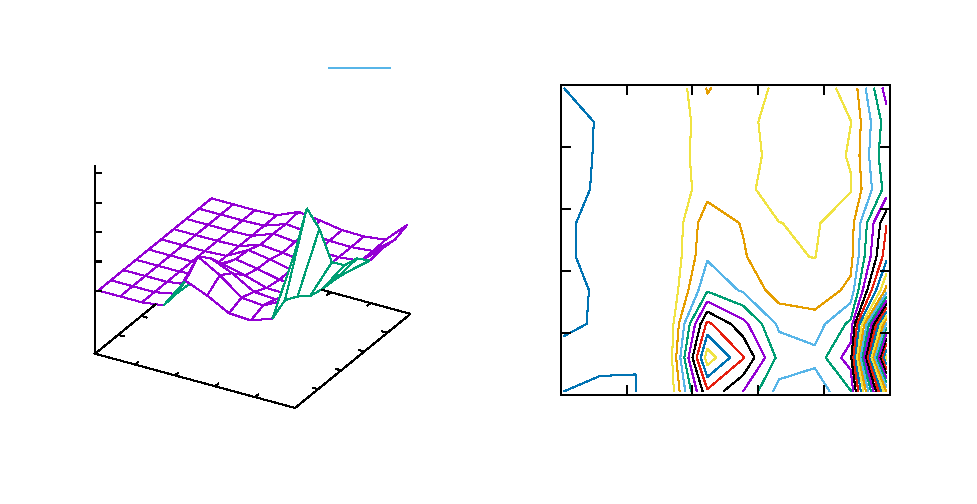
\includegraphics{images/plots/plot_11_40_1000}}%
    \gplfronttext
  \end{picture}%
\endgroup
}
	\caption{ Плотность распределения указанной копулы}
	\label{fig:smallxm}
\end{figure}
На рисунке \ref{fig:smallxm} приведена плотность копулы, соответствующей оценкам вероятностей попадания модельных значений параметров $\sigma$ и $x_m$ в построенные для них интервалы.
Максимум в нижней части контурного графика наталкивает на мысль, что нужно провести исследование того подмножества модельных наборов параметров, который приводит к такой картине. Это всего лишь одно из непосредственных возможных применений построенных оценок в форме копул.

\begin{figure}[h]
	{% GNUPLOT: LaTeX picture with Postscript
\begingroup
  \makeatletter
  \providecommand\color[2][]{%
    \GenericError{(gnuplot) \space\space\space\@spaces}{%
      Package color not loaded in conjunction with
      terminal option `colourtext'%
    }{See the gnuplot documentation for explanation.%
    }{Either use 'blacktext' in gnuplot or load the package
      color.sty in LaTeX.}%
    \renewcommand\color[2][]{}%
  }%
  \providecommand\includegraphics[2][]{%
    \GenericError{(gnuplot) \space\space\space\@spaces}{%
      Package graphicx or graphics not loaded%
    }{See the gnuplot documentation for explanation.%
    }{The gnuplot epslatex terminal needs graphicx.sty or graphics.sty.}%
    \renewcommand\includegraphics[2][]{}%
  }%
  \providecommand\rotatebox[2]{#2}%
  \@ifundefined{ifGPcolor}{%
    \newif\ifGPcolor
    \GPcolortrue
  }{}%
  \@ifundefined{ifGPblacktext}{%
    \newif\ifGPblacktext
    \GPblacktextfalse
  }{}%
  % define a \g@addto@macro without @ in the name:
  \let\gplgaddtomacro\g@addto@macro
  % define empty templates for all commands taking text:
  \gdef\gplbacktext{}%
  \gdef\gplfronttext{}%
  \makeatother
  \ifGPblacktext
    % no textcolor at all
    \def\colorrgb#1{}%
    \def\colorgray#1{}%
  \else
    % gray or color?
    \ifGPcolor
      \def\colorrgb#1{\color[rgb]{#1}}%
      \def\colorgray#1{\color[gray]{#1}}%
      \expandafter\def\csname LTw\endcsname{\color{white}}%
      \expandafter\def\csname LTb\endcsname{\color{black}}%
      \expandafter\def\csname LTa\endcsname{\color{black}}%
      \expandafter\def\csname LT0\endcsname{\color[rgb]{1,0,0}}%
      \expandafter\def\csname LT1\endcsname{\color[rgb]{0,1,0}}%
      \expandafter\def\csname LT2\endcsname{\color[rgb]{0,0,1}}%
      \expandafter\def\csname LT3\endcsname{\color[rgb]{1,0,1}}%
      \expandafter\def\csname LT4\endcsname{\color[rgb]{0,1,1}}%
      \expandafter\def\csname LT5\endcsname{\color[rgb]{1,1,0}}%
      \expandafter\def\csname LT6\endcsname{\color[rgb]{0,0,0}}%
      \expandafter\def\csname LT7\endcsname{\color[rgb]{1,0.3,0}}%
      \expandafter\def\csname LT8\endcsname{\color[rgb]{0.5,0.5,0.5}}%
    \else
      % gray
      \def\colorrgb#1{\color{black}}%
      \def\colorgray#1{\color[gray]{#1}}%
      \expandafter\def\csname LTw\endcsname{\color{white}}%
      \expandafter\def\csname LTb\endcsname{\color{black}}%
      \expandafter\def\csname LTa\endcsname{\color{black}}%
      \expandafter\def\csname LT0\endcsname{\color{black}}%
      \expandafter\def\csname LT1\endcsname{\color{black}}%
      \expandafter\def\csname LT2\endcsname{\color{black}}%
      \expandafter\def\csname LT3\endcsname{\color{black}}%
      \expandafter\def\csname LT4\endcsname{\color{black}}%
      \expandafter\def\csname LT5\endcsname{\color{black}}%
      \expandafter\def\csname LT6\endcsname{\color{black}}%
      \expandafter\def\csname LT7\endcsname{\color{black}}%
      \expandafter\def\csname LT8\endcsname{\color{black}}%
    \fi
  \fi
    \setlength{\unitlength}{0.0500bp}%
    \ifx\gptboxheight\undefined%
      \newlength{\gptboxheight}%
      \newlength{\gptboxwidth}%
      \newsavebox{\gptboxtext}%
    \fi%
    \setlength{\fboxrule}{0.5pt}%
    \setlength{\fboxsep}{1pt}%
\begin{picture}(4534.00,5668.00)%
    \gplgaddtomacro\gplbacktext{%
      \colorrgb{0.00,0.00,0.00}%
      \put(924,3714){\makebox(0,0)[r]{\strut{}\ft $0$}}%
      \colorrgb{0.00,0.00,0.00}%
      \put(924,3939){\makebox(0,0)[r]{\strut{}\ft $0.2$}}%
      \colorrgb{0.00,0.00,0.00}%
      \put(924,4164){\makebox(0,0)[r]{\strut{}\ft $0.4$}}%
      \colorrgb{0.00,0.00,0.00}%
      \put(924,4390){\makebox(0,0)[r]{\strut{}\ft $0.6$}}%
      \colorrgb{0.00,0.00,0.00}%
      \put(924,4615){\makebox(0,0)[r]{\strut{}\ft $0.8$}}%
      \colorrgb{0.00,0.00,0.00}%
      \put(924,4840){\makebox(0,0)[r]{\strut{}\ft $1$}}%
      \colorrgb{0.00,0.00,0.00}%
      \put(924,5065){\makebox(0,0)[r]{\strut{}\ft $1.2$}}%
      \colorrgb{0.00,0.00,0.00}%
      \put(924,5290){\makebox(0,0)[r]{\strut{}\ft $1.4$}}%
      \colorrgb{0.00,0.00,0.00}%
      \put(1364,3494){\makebox(0,0){\strut{}\ft $-4$}}%
      \colorrgb{0.00,0.00,0.00}%
      \put(1980,3494){\makebox(0,0){\strut{}\ft $-2$}}%
      \colorrgb{0.00,0.00,0.00}%
      \put(2597,3494){\makebox(0,0){\strut{}\ft $0$}}%
      \colorrgb{0.00,0.00,0.00}%
      \put(3213,3494){\makebox(0,0){\strut{}\ft $2$}}%
      \colorrgb{0.00,0.00,0.00}%
      \put(3829,3494){\makebox(0,0){\strut{}\ft $4$}}%
      \colorrgb{0.00,0.00,0.00}%
      \put(2597,3054){\makebox(0,0){\strut{}$Z(t), Y(t)$}}%
      \put(2597,6063){\makebox(0,0){\strut{}}}%
      \put(132,4559){\rotatebox{90}{\makebox(0,0){\strut{}$f(X(t)), f(Y(t))$}}}%
      \put(4401,4559){\rotatebox{90}{\makebox(0,0){\strut{}}}}%
    }%
    \gplgaddtomacro\gplfronttext{%
      \colorrgb{0.00,0.00,0.00}%
      \put(242,4558){\rotatebox{-270}{\makebox(0,0){\strut{}}}}%
      \colorrgb{0.00,0.00,0.00}%
      \put(2596,3208){\makebox(0,0){\strut{}}}%
    }%
    \gplbacktext
    \put(0,0){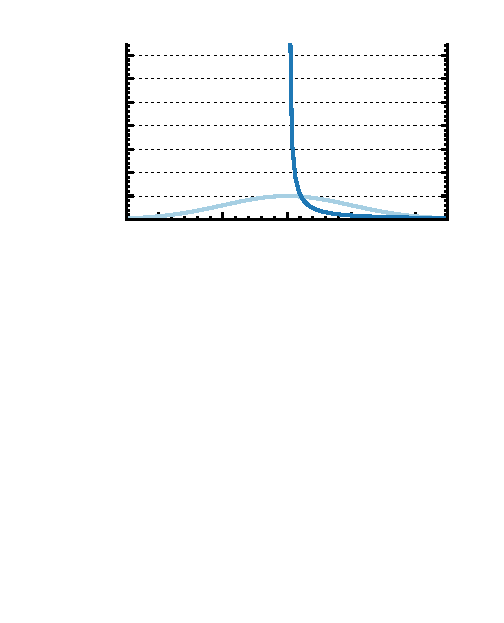
\includegraphics{ZY}}%
    \gplfronttext
  \end{picture}%
\endgroup
}
	\caption{Плотности распределения указанных процессов при фиксированном $t$}
	\label{fig:zy}
\end{figure}
На рисунке синим изображена плотность распределения Y(t). При увеличении модельного значения $x_m$ она сдвигается вправо, отдаляясь от моды распределения $Z(t)$. С теоретической точки зрения, это должно обеспечивать условия, при которых вероятность построения границ компактов будет выше, алгоритм интервального оценивания будет доставлять лучшие результаты.


\begin{figure}[H]
	{% GNUPLOT: LaTeX picture with Postscript
\begingroup
  \makeatletter
  \providecommand\color[2][]{%
    \GenericError{(gnuplot) \space\space\space\@spaces}{%
      Package color not loaded in conjunction with
      terminal option `colourtext'%
    }{See the gnuplot documentation for explanation.%
    }{Either use 'blacktext' in gnuplot or load the package
      color.sty in LaTeX.}%
    \renewcommand\color[2][]{}%
  }%
  \providecommand\includegraphics[2][]{%
    \GenericError{(gnuplot) \space\space\space\@spaces}{%
      Package graphicx or graphics not loaded%
    }{See the gnuplot documentation for explanation.%
    }{The gnuplot epslatex terminal needs graphicx.sty or graphics.sty.}%
    \renewcommand\includegraphics[2][]{}%
  }%
  \providecommand\rotatebox[2]{#2}%
  \@ifundefined{ifGPcolor}{%
    \newif\ifGPcolor
    \GPcolortrue
  }{}%
  \@ifundefined{ifGPblacktext}{%
    \newif\ifGPblacktext
    \GPblacktextfalse
  }{}%
  % define a \g@addto@macro without @ in the name:
  \let\gplgaddtomacro\g@addto@macro
  % define empty templates for all commands taking text:
  \gdef\gplbacktext{}%
  \gdef\gplfronttext{}%
  \makeatother
  \ifGPblacktext
    % no textcolor at all
    \def\colorrgb#1{}%
    \def\colorgray#1{}%
  \else
    % gray or color?
    \ifGPcolor
      \def\colorrgb#1{\color[rgb]{#1}}%
      \def\colorgray#1{\color[gray]{#1}}%
      \expandafter\def\csname LTw\endcsname{\color{white}}%
      \expandafter\def\csname LTb\endcsname{\color{black}}%
      \expandafter\def\csname LTa\endcsname{\color{black}}%
      \expandafter\def\csname LT0\endcsname{\color[rgb]{1,0,0}}%
      \expandafter\def\csname LT1\endcsname{\color[rgb]{0,1,0}}%
      \expandafter\def\csname LT2\endcsname{\color[rgb]{0,0,1}}%
      \expandafter\def\csname LT3\endcsname{\color[rgb]{1,0,1}}%
      \expandafter\def\csname LT4\endcsname{\color[rgb]{0,1,1}}%
      \expandafter\def\csname LT5\endcsname{\color[rgb]{1,1,0}}%
      \expandafter\def\csname LT6\endcsname{\color[rgb]{0,0,0}}%
      \expandafter\def\csname LT7\endcsname{\color[rgb]{1,0.3,0}}%
      \expandafter\def\csname LT8\endcsname{\color[rgb]{0.5,0.5,0.5}}%
    \else
      % gray
      \def\colorrgb#1{\color{black}}%
      \def\colorgray#1{\color[gray]{#1}}%
      \expandafter\def\csname LTw\endcsname{\color{white}}%
      \expandafter\def\csname LTb\endcsname{\color{black}}%
      \expandafter\def\csname LTa\endcsname{\color{black}}%
      \expandafter\def\csname LT0\endcsname{\color{black}}%
      \expandafter\def\csname LT1\endcsname{\color{black}}%
      \expandafter\def\csname LT2\endcsname{\color{black}}%
      \expandafter\def\csname LT3\endcsname{\color{black}}%
      \expandafter\def\csname LT4\endcsname{\color{black}}%
      \expandafter\def\csname LT5\endcsname{\color{black}}%
      \expandafter\def\csname LT6\endcsname{\color{black}}%
      \expandafter\def\csname LT7\endcsname{\color{black}}%
      \expandafter\def\csname LT8\endcsname{\color{black}}%
    \fi
  \fi
    \setlength{\unitlength}{0.0500bp}%
    \ifx\gptboxheight\undefined%
      \newlength{\gptboxheight}%
      \newlength{\gptboxwidth}%
      \newsavebox{\gptboxtext}%
    \fi%
    \setlength{\fboxrule}{0.5pt}%
    \setlength{\fboxsep}{1pt}%
\begin{picture}(9070.00,4534.00)%
    \gplgaddtomacro\gplbacktext{%
    }%
    \gplgaddtomacro\gplfronttext{%
      \csname LTb\endcsname%
      \put(2863,4030){\makebox(0,0)[r]{\strut{}$\widehat{p}_\sigma=2.12132$, $\widehat{p}_\lambda=100$}}%
      \csname LTb\endcsname%
      \put(683,1188){\makebox(0,0){\strut{}\ft $0$}}%
      \put(1067,1084){\makebox(0,0){\strut{}\ft $0.2$}}%
      \put(1451,979){\makebox(0,0){\strut{}\ft $0.4$}}%
      \put(1835,875){\makebox(0,0){\strut{}\ft $0.6$}}%
      \put(2219,771){\makebox(0,0){\strut{}\ft $0.8$}}%
      \put(2602,667){\makebox(0,0){\strut{}\ft $1$}}%
      \put(1436,797){\makebox(0,0){\strut{}$\widehat{p}_\sigma$}}%
      \put(2787,710){\makebox(0,0){\strut{}\ft $0$}}%
      \put(3008,891){\makebox(0,0){\strut{}\ft $0.2$}}%
      \put(3230,1071){\makebox(0,0){\strut{}\ft $0.4$}}%
      \put(3452,1252){\makebox(0,0){\strut{}\ft $0.6$}}%
      \put(3673,1433){\makebox(0,0){\strut{}\ft $0.8$}}%
      \put(3895,1613){\makebox(0,0){\strut{}\ft $1$}}%
      \put(3706,1083){\makebox(0,0){\strut{}$\widehat{p}_\lambda$}}%
      \put(627,1885){\makebox(0,0)[r]{\strut{}\ft $0$}}%
      \put(627,2831){\makebox(0,0)[r]{\strut{}\ft $3$}}%
      \put(-171,2487){\makebox(0,0){\strut{}$\widehat{c}$}}%
    }%
    \gplgaddtomacro\gplbacktext{%
    }%
    \gplgaddtomacro\gplfronttext{%
      \csname LTb\endcsname%
      \put(5223,578){\makebox(0,0){\strut{}\ft $0$}}%
      \put(5855,578){\makebox(0,0){\strut{}\ft $0.2$}}%
      \put(6487,578){\makebox(0,0){\strut{}\ft $0.4$}}%
      \put(7117,578){\makebox(0,0){\strut{}\ft $0.6$}}%
      \put(7749,578){\makebox(0,0){\strut{}\ft $0.8$}}%
      \put(8381,578){\makebox(0,0){\strut{}\ft $1$}}%
      \put(6802,248){\makebox(0,0){\strut{}$\widehat{p}_\sigma$}}%
      \put(5035,891){\makebox(0,0)[r]{\strut{}\ft $0$}}%
      \put(5035,1486){\makebox(0,0)[r]{\strut{}\ft $0.2$}}%
      \put(5035,2080){\makebox(0,0)[r]{\strut{}\ft $0.4$}}%
      \put(5035,2674){\makebox(0,0)[r]{\strut{}\ft $0.6$}}%
      \put(5035,3268){\makebox(0,0)[r]{\strut{}\ft $0.8$}}%
      \put(5035,3863){\makebox(0,0)[r]{\strut{}\ft $1$}}%
      \put(4309,2377){\rotatebox{-270}{\makebox(0,0){\strut{}$\widehat{p}_\lambda$}}}%
    }%
    \gplbacktext
    \put(0,0){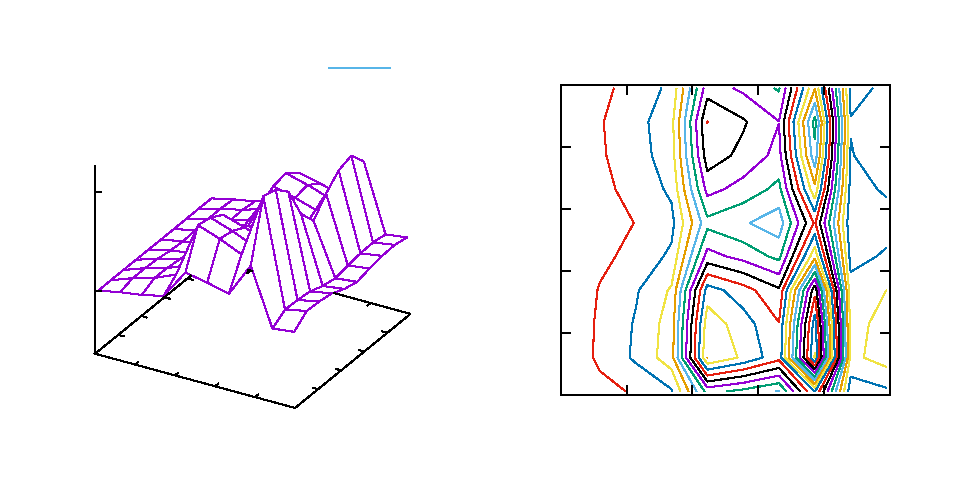
\includegraphics{images/plots/plot_11_41_1000}}%
    \gplfronttext
  \end{picture}%
\endgroup
}
	\caption{Плотность распределения указанной копулы}
	\label{fig:bigxm}
\end{figure}
На рисунке \ref{fig:bigxm} приведена плотность копулы, соответствующей тем же оценкам, но с большим значением $x_m$. Максимум в верхней правой части означает, что алгоритм интервального оценивания успешно справляется со своей задачей, когда модельное значение $x_m$ увеличивается. Это подтверждает априорные теоретически обоснованные предположения, иллюстрируемые на \ref{fig:zy}. Можно построить вероятностную меру, количественно оценивающую связь между соотношением  модельных значений $x_m$ и $\sigma$ и вероятностью успеха  алгоритма интервального оценивания.

Таким образом
\begin{itemize}
  \item Форма копулы подтвердила априорные предположения о характере связи оценок $\sigma$ и $x_m$;
  \item Локальный экстремум в этой части носителя меры копулы  (при малом модельном значении $x_m$) даёт формально обоснованный повод для проведения дальнейших исследований алгоритма построения границ компакта, причём копула обеспечивает нас информацией о том, на каком подмножестве пар значений параметров сигма и $x_m$ следует сосредоточить внимание.
\end{itemize}

Рассмотрим теперь пару $\sigma$, $\lambda$.
\begin{figure}[H]
	{% GNUPLOT: LaTeX picture with Postscript
\begingroup
  \makeatletter
  \providecommand\color[2][]{%
    \GenericError{(gnuplot) \space\space\space\@spaces}{%
      Package color not loaded in conjunction with
      terminal option `colourtext'%
    }{See the gnuplot documentation for explanation.%
    }{Either use 'blacktext' in gnuplot or load the package
      color.sty in LaTeX.}%
    \renewcommand\color[2][]{}%
  }%
  \providecommand\includegraphics[2][]{%
    \GenericError{(gnuplot) \space\space\space\@spaces}{%
      Package graphicx or graphics not loaded%
    }{See the gnuplot documentation for explanation.%
    }{The gnuplot epslatex terminal needs graphicx.sty or graphics.sty.}%
    \renewcommand\includegraphics[2][]{}%
  }%
  \providecommand\rotatebox[2]{#2}%
  \@ifundefined{ifGPcolor}{%
    \newif\ifGPcolor
    \GPcolortrue
  }{}%
  \@ifundefined{ifGPblacktext}{%
    \newif\ifGPblacktext
    \GPblacktextfalse
  }{}%
  % define a \g@addto@macro without @ in the name:
  \let\gplgaddtomacro\g@addto@macro
  % define empty templates for all commands taking text:
  \gdef\gplbacktext{}%
  \gdef\gplfronttext{}%
  \makeatother
  \ifGPblacktext
    % no textcolor at all
    \def\colorrgb#1{}%
    \def\colorgray#1{}%
  \else
    % gray or color?
    \ifGPcolor
      \def\colorrgb#1{\color[rgb]{#1}}%
      \def\colorgray#1{\color[gray]{#1}}%
      \expandafter\def\csname LTw\endcsname{\color{white}}%
      \expandafter\def\csname LTb\endcsname{\color{black}}%
      \expandafter\def\csname LTa\endcsname{\color{black}}%
      \expandafter\def\csname LT0\endcsname{\color[rgb]{1,0,0}}%
      \expandafter\def\csname LT1\endcsname{\color[rgb]{0,1,0}}%
      \expandafter\def\csname LT2\endcsname{\color[rgb]{0,0,1}}%
      \expandafter\def\csname LT3\endcsname{\color[rgb]{1,0,1}}%
      \expandafter\def\csname LT4\endcsname{\color[rgb]{0,1,1}}%
      \expandafter\def\csname LT5\endcsname{\color[rgb]{1,1,0}}%
      \expandafter\def\csname LT6\endcsname{\color[rgb]{0,0,0}}%
      \expandafter\def\csname LT7\endcsname{\color[rgb]{1,0.3,0}}%
      \expandafter\def\csname LT8\endcsname{\color[rgb]{0.5,0.5,0.5}}%
    \else
      % gray
      \def\colorrgb#1{\color{black}}%
      \def\colorgray#1{\color[gray]{#1}}%
      \expandafter\def\csname LTw\endcsname{\color{white}}%
      \expandafter\def\csname LTb\endcsname{\color{black}}%
      \expandafter\def\csname LTa\endcsname{\color{black}}%
      \expandafter\def\csname LT0\endcsname{\color{black}}%
      \expandafter\def\csname LT1\endcsname{\color{black}}%
      \expandafter\def\csname LT2\endcsname{\color{black}}%
      \expandafter\def\csname LT3\endcsname{\color{black}}%
      \expandafter\def\csname LT4\endcsname{\color{black}}%
      \expandafter\def\csname LT5\endcsname{\color{black}}%
      \expandafter\def\csname LT6\endcsname{\color{black}}%
      \expandafter\def\csname LT7\endcsname{\color{black}}%
      \expandafter\def\csname LT8\endcsname{\color{black}}%
    \fi
  \fi
    \setlength{\unitlength}{0.0500bp}%
    \ifx\gptboxheight\undefined%
      \newlength{\gptboxheight}%
      \newlength{\gptboxwidth}%
      \newsavebox{\gptboxtext}%
    \fi%
    \setlength{\fboxrule}{0.5pt}%
    \setlength{\fboxsep}{1pt}%
\begin{picture}(9070.00,4534.00)%
    \gplgaddtomacro\gplbacktext{%
    }%
    \gplgaddtomacro\gplfronttext{%
      \csname LTb\endcsname%
      \put(2863,4030){\makebox(0,0)[r]{\strut{}$\sigma=0.707107$, $x_m=0.01$}}%
      \csname LTb\endcsname%
      \put(683,1188){\makebox(0,0){\strut{}\ft $0$}}%
      \put(1067,1084){\makebox(0,0){\strut{}\ft $0.2$}}%
      \put(1451,979){\makebox(0,0){\strut{}\ft $0.4$}}%
      \put(1835,875){\makebox(0,0){\strut{}\ft $0.6$}}%
      \put(2219,771){\makebox(0,0){\strut{}\ft $0.8$}}%
      \put(2602,667){\makebox(0,0){\strut{}\ft $1$}}%
      \put(1436,797){\makebox(0,0){\strut{}$\widehat{p}_\sigma$}}%
      \put(2787,710){\makebox(0,0){\strut{}\ft $0$}}%
      \put(3008,891){\makebox(0,0){\strut{}\ft $0.2$}}%
      \put(3230,1071){\makebox(0,0){\strut{}\ft $0.4$}}%
      \put(3452,1252){\makebox(0,0){\strut{}\ft $0.6$}}%
      \put(3673,1433){\makebox(0,0){\strut{}\ft $0.8$}}%
      \put(3895,1613){\makebox(0,0){\strut{}\ft $1$}}%
      \put(3706,1083){\makebox(0,0){\strut{}$\widehat{p}_{x_m}$}}%
      \put(627,1886){\makebox(0,0)[r]{\strut{}\ft $0$}}%
      \put(627,2115){\makebox(0,0)[r]{\strut{}\ft $10$}}%
      \put(627,2344){\makebox(0,0)[r]{\strut{}\ft $20$}}%
      \put(627,2572){\makebox(0,0)[r]{\strut{}\ft $30$}}%
      \put(627,2802){\makebox(0,0)[r]{\strut{}\ft $40$}}%
      \put(627,3031){\makebox(0,0)[r]{\strut{}\ft $50$}}%
      \put(-171,2487){\makebox(0,0){\strut{}$\widehat{c}$}}%
    }%
    \gplgaddtomacro\gplbacktext{%
    }%
    \gplgaddtomacro\gplfronttext{%
      \csname LTb\endcsname%
      \put(5223,578){\makebox(0,0){\strut{}\ft $0$}}%
      \put(5855,578){\makebox(0,0){\strut{}\ft $0.2$}}%
      \put(6487,578){\makebox(0,0){\strut{}\ft $0.4$}}%
      \put(7117,578){\makebox(0,0){\strut{}\ft $0.6$}}%
      \put(7749,578){\makebox(0,0){\strut{}\ft $0.8$}}%
      \put(8381,578){\makebox(0,0){\strut{}\ft $1$}}%
      \put(6802,248){\makebox(0,0){\strut{}$\widehat{p}_\sigma$}}%
      \put(5035,891){\makebox(0,0)[r]{\strut{}\ft $0$}}%
      \put(5035,1486){\makebox(0,0)[r]{\strut{}\ft $0.2$}}%
      \put(5035,2080){\makebox(0,0)[r]{\strut{}\ft $0.4$}}%
      \put(5035,2674){\makebox(0,0)[r]{\strut{}\ft $0.6$}}%
      \put(5035,3268){\makebox(0,0)[r]{\strut{}\ft $0.8$}}%
      \put(5035,3863){\makebox(0,0)[r]{\strut{}\ft $1$}}%
      \put(4309,2377){\rotatebox{-270}{\makebox(0,0){\strut{}$\widehat{p}_{x_m}$}}}%
    }%
    \gplbacktext
    \put(0,0){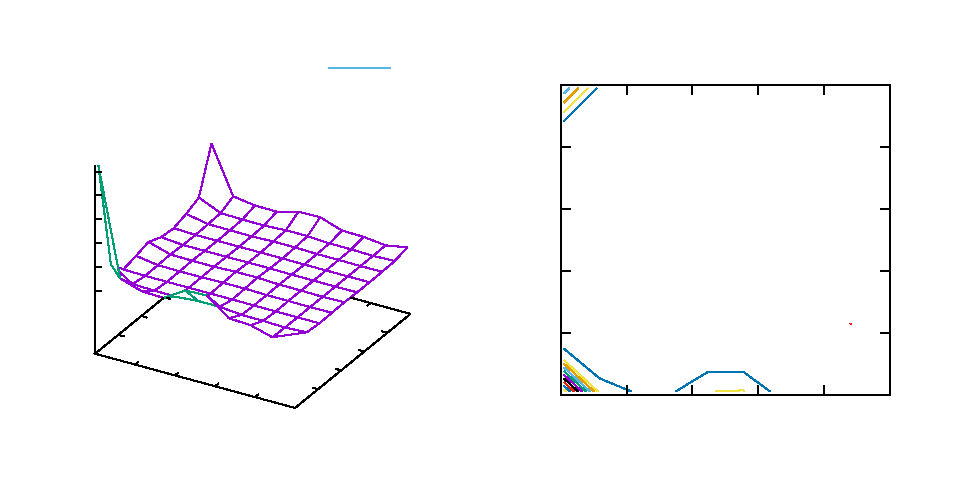
\includegraphics{plot_10_20_1000}}%
    \gplfronttext
  \end{picture}%
\endgroup
}
	\caption{Плотность распределения указанной копулы}
	\label{fig:smalllambda}
\end{figure}
Параметр $\lambda$ определяет интенсивность потока пуассоновских событий. На рисунке \ref{fig:smalllambda} увеличение значения оценки копулы при вероятности правильной оценки $\lambda$, близкой к 1, можно интерпретировать как успешную идентификацию всех выбросов. А значит выборка для оценки границ компакта для $x_m$ построена успешно.

Увеличение значения оценки копулы при вероятности правильной оценки $\lambda$, близкой к 0, сейчас откровенно озадачивает.

\begin{figure}[H]
	{% GNUPLOT: LaTeX picture with Postscript
\begingroup
  \makeatletter
  \providecommand\color[2][]{%
    \GenericError{(gnuplot) \space\space\space\@spaces}{%
      Package color not loaded in conjunction with
      terminal option `colourtext'%
    }{See the gnuplot documentation for explanation.%
    }{Either use 'blacktext' in gnuplot or load the package
      color.sty in LaTeX.}%
    \renewcommand\color[2][]{}%
  }%
  \providecommand\includegraphics[2][]{%
    \GenericError{(gnuplot) \space\space\space\@spaces}{%
      Package graphicx or graphics not loaded%
    }{See the gnuplot documentation for explanation.%
    }{The gnuplot epslatex terminal needs graphicx.sty or graphics.sty.}%
    \renewcommand\includegraphics[2][]{}%
  }%
  \providecommand\rotatebox[2]{#2}%
  \@ifundefined{ifGPcolor}{%
    \newif\ifGPcolor
    \GPcolortrue
  }{}%
  \@ifundefined{ifGPblacktext}{%
    \newif\ifGPblacktext
    \GPblacktextfalse
  }{}%
  % define a \g@addto@macro without @ in the name:
  \let\gplgaddtomacro\g@addto@macro
  % define empty templates for all commands taking text:
  \gdef\gplbacktext{}%
  \gdef\gplfronttext{}%
  \makeatother
  \ifGPblacktext
    % no textcolor at all
    \def\colorrgb#1{}%
    \def\colorgray#1{}%
  \else
    % gray or color?
    \ifGPcolor
      \def\colorrgb#1{\color[rgb]{#1}}%
      \def\colorgray#1{\color[gray]{#1}}%
      \expandafter\def\csname LTw\endcsname{\color{white}}%
      \expandafter\def\csname LTb\endcsname{\color{black}}%
      \expandafter\def\csname LTa\endcsname{\color{black}}%
      \expandafter\def\csname LT0\endcsname{\color[rgb]{1,0,0}}%
      \expandafter\def\csname LT1\endcsname{\color[rgb]{0,1,0}}%
      \expandafter\def\csname LT2\endcsname{\color[rgb]{0,0,1}}%
      \expandafter\def\csname LT3\endcsname{\color[rgb]{1,0,1}}%
      \expandafter\def\csname LT4\endcsname{\color[rgb]{0,1,1}}%
      \expandafter\def\csname LT5\endcsname{\color[rgb]{1,1,0}}%
      \expandafter\def\csname LT6\endcsname{\color[rgb]{0,0,0}}%
      \expandafter\def\csname LT7\endcsname{\color[rgb]{1,0.3,0}}%
      \expandafter\def\csname LT8\endcsname{\color[rgb]{0.5,0.5,0.5}}%
    \else
      % gray
      \def\colorrgb#1{\color{black}}%
      \def\colorgray#1{\color[gray]{#1}}%
      \expandafter\def\csname LTw\endcsname{\color{white}}%
      \expandafter\def\csname LTb\endcsname{\color{black}}%
      \expandafter\def\csname LTa\endcsname{\color{black}}%
      \expandafter\def\csname LT0\endcsname{\color{black}}%
      \expandafter\def\csname LT1\endcsname{\color{black}}%
      \expandafter\def\csname LT2\endcsname{\color{black}}%
      \expandafter\def\csname LT3\endcsname{\color{black}}%
      \expandafter\def\csname LT4\endcsname{\color{black}}%
      \expandafter\def\csname LT5\endcsname{\color{black}}%
      \expandafter\def\csname LT6\endcsname{\color{black}}%
      \expandafter\def\csname LT7\endcsname{\color{black}}%
      \expandafter\def\csname LT8\endcsname{\color{black}}%
    \fi
  \fi
    \setlength{\unitlength}{0.0500bp}%
    \ifx\gptboxheight\undefined%
      \newlength{\gptboxheight}%
      \newlength{\gptboxwidth}%
      \newsavebox{\gptboxtext}%
    \fi%
    \setlength{\fboxrule}{0.5pt}%
    \setlength{\fboxsep}{1pt}%
\begin{picture}(9070.00,4534.00)%
    \gplgaddtomacro\gplbacktext{%
    }%
    \gplgaddtomacro\gplfronttext{%
      \csname LTb\endcsname%
      \put(2863,4030){\makebox(0,0)[r]{\strut{}$\widehat{p}_\sigma=0.707107$, $\widehat{p}_{x_m}=0.125$}}%
      \csname LTb\endcsname%
      \put(683,1188){\makebox(0,0){\strut{}\ft $0$}}%
      \put(1067,1084){\makebox(0,0){\strut{}\ft $0.2$}}%
      \put(1451,979){\makebox(0,0){\strut{}\ft $0.4$}}%
      \put(1835,875){\makebox(0,0){\strut{}\ft $0.6$}}%
      \put(2219,771){\makebox(0,0){\strut{}\ft $0.8$}}%
      \put(2602,667){\makebox(0,0){\strut{}\ft $1$}}%
      \put(1436,797){\makebox(0,0){\strut{}$\widehat{p}_\sigma$}}%
      \put(2787,710){\makebox(0,0){\strut{}\ft $0$}}%
      \put(3008,891){\makebox(0,0){\strut{}\ft $0.2$}}%
      \put(3230,1071){\makebox(0,0){\strut{}\ft $0.4$}}%
      \put(3452,1252){\makebox(0,0){\strut{}\ft $0.6$}}%
      \put(3673,1433){\makebox(0,0){\strut{}\ft $0.8$}}%
      \put(3895,1613){\makebox(0,0){\strut{}\ft $1$}}%
      \put(3706,1083){\makebox(0,0){\strut{}$\widehat{p}_{x_m}$}}%
      \put(627,1886){\makebox(0,0)[r]{\strut{}\ft $0$}}%
      \put(627,1920){\makebox(0,0)[r]{\strut{}\ft $3$}}%
      \put(627,1955){\makebox(0,0)[r]{\strut{}\ft $6$}}%
      \put(627,1990){\makebox(0,0)[r]{\strut{}\ft $9$}}%
      \put(627,2024){\makebox(0,0)[r]{\strut{}\ft $12$}}%
      \put(627,2059){\makebox(0,0)[r]{\strut{}\ft $15$}}%
      \put(627,2094){\makebox(0,0)[r]{\strut{}\ft $18$}}%
      \put(627,2129){\makebox(0,0)[r]{\strut{}\ft $21$}}%
      \put(627,2163){\makebox(0,0)[r]{\strut{}\ft $24$}}%
      \put(627,2198){\makebox(0,0)[r]{\strut{}\ft $27$}}%
      \put(627,2233){\makebox(0,0)[r]{\strut{}\ft $30$}}%
      \put(627,2267){\makebox(0,0)[r]{\strut{}\ft $33$}}%
      \put(627,2302){\makebox(0,0)[r]{\strut{}\ft $36$}}%
      \put(627,2337){\makebox(0,0)[r]{\strut{}\ft $39$}}%
      \put(627,2372){\makebox(0,0)[r]{\strut{}\ft $42$}}%
      \put(627,2405){\makebox(0,0)[r]{\strut{}\ft $45$}}%
      \put(627,2440){\makebox(0,0)[r]{\strut{}\ft $48$}}%
      \put(627,2475){\makebox(0,0)[r]{\strut{}\ft $51$}}%
      \put(627,2510){\makebox(0,0)[r]{\strut{}\ft $54$}}%
      \put(627,2544){\makebox(0,0)[r]{\strut{}\ft $57$}}%
      \put(627,2579){\makebox(0,0)[r]{\strut{}\ft $60$}}%
      \put(627,2614){\makebox(0,0)[r]{\strut{}\ft $63$}}%
      \put(627,2648){\makebox(0,0)[r]{\strut{}\ft $66$}}%
      \put(627,2683){\makebox(0,0)[r]{\strut{}\ft $69$}}%
      \put(627,2718){\makebox(0,0)[r]{\strut{}\ft $72$}}%
      \put(627,2753){\makebox(0,0)[r]{\strut{}\ft $75$}}%
      \put(627,2787){\makebox(0,0)[r]{\strut{}\ft $78$}}%
      \put(627,2822){\makebox(0,0)[r]{\strut{}\ft $81$}}%
      \put(627,2857){\makebox(0,0)[r]{\strut{}\ft $84$}}%
      \put(627,2891){\makebox(0,0)[r]{\strut{}\ft $87$}}%
      \put(627,2926){\makebox(0,0)[r]{\strut{}\ft $90$}}%
      \put(627,2961){\makebox(0,0)[r]{\strut{}\ft $93$}}%
      \put(627,2996){\makebox(0,0)[r]{\strut{}\ft $96$}}%
      \put(627,3030){\makebox(0,0)[r]{\strut{}\ft $99$}}%
      \put(627,3065){\makebox(0,0)[r]{\strut{}\ft $102$}}%
      \put(-171,2487){\makebox(0,0){\strut{}$\widehat{c}$}}%
    }%
    \gplgaddtomacro\gplbacktext{%
    }%
    \gplgaddtomacro\gplfronttext{%
      \csname LTb\endcsname%
      \put(5223,578){\makebox(0,0){\strut{}\ft $0$}}%
      \put(5855,578){\makebox(0,0){\strut{}\ft $0.2$}}%
      \put(6487,578){\makebox(0,0){\strut{}\ft $0.4$}}%
      \put(7117,578){\makebox(0,0){\strut{}\ft $0.6$}}%
      \put(7749,578){\makebox(0,0){\strut{}\ft $0.8$}}%
      \put(8381,578){\makebox(0,0){\strut{}\ft $1$}}%
      \put(6802,248){\makebox(0,0){\strut{}$\widehat{p}_\sigma$}}%
      \put(5035,891){\makebox(0,0)[r]{\strut{}\ft $0$}}%
      \put(5035,1486){\makebox(0,0)[r]{\strut{}\ft $0.2$}}%
      \put(5035,2080){\makebox(0,0)[r]{\strut{}\ft $0.4$}}%
      \put(5035,2674){\makebox(0,0)[r]{\strut{}\ft $0.6$}}%
      \put(5035,3268){\makebox(0,0)[r]{\strut{}\ft $0.8$}}%
      \put(5035,3863){\makebox(0,0)[r]{\strut{}\ft $1$}}%
      \put(4309,2377){\rotatebox{-270}{\makebox(0,0){\strut{}$\widehat{p}_{x_m}$}}}%
    }%
    \gplbacktext
    \put(0,0){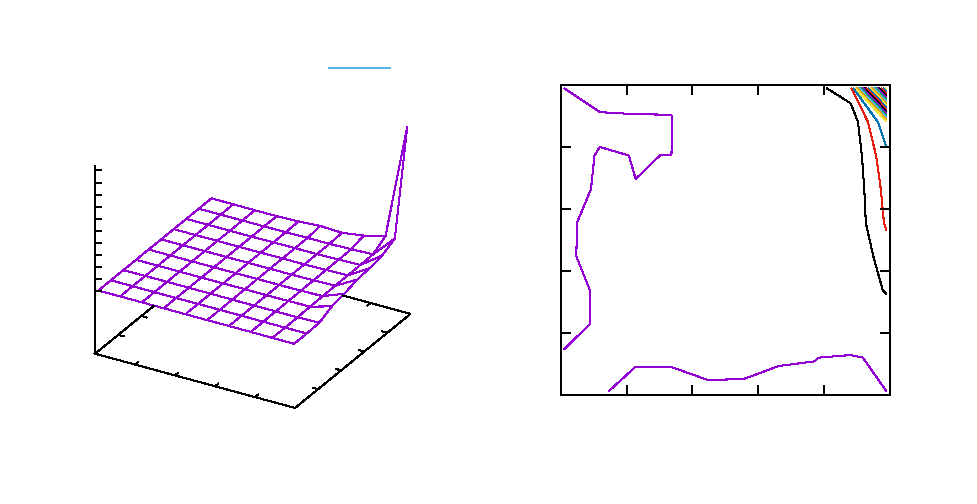
\includegraphics{images/plots/plot_10_21_1000}}%
    \gplfronttext
  \end{picture}%
\endgroup
}
	\caption{Плотность распределения указанной копулы}
	\label{fig:biglambda}
\end{figure}
Копула на рисунке \ref{fig:biglambda} также соответствует модели процесса $X(t)$.

Таким образом форма копулы также подтвердила априорные предположения о характере связи оценок $\sigma$ и $\lambda$.

\clearpage
